%!TEX root = ../thesis.tex
%*******************************************************************************
%*********************************** Forth Chapter *****************************
%*******************************************************************************

\chapter{Numerical Tests and Results}  %Title of the Forth Chapter

\ifpdf
    \graphicspath{{Chapter4/Figs/PDF/}{Chapter4/Figs/}}
\else
    \graphicspath{{Chapter4/Figs/}}
\fi


%********************************** %First Section  **************************************
\section{Multigrid solver tests} %Section - 4.1 
\label{section4.1}
\subsection{Newtonian gravitational field}
For simplicity, we consider only the test of Poisson equation.
In Newtonian gravity, the gravitational potential $\Phi$ can be obtained by
\begin{align}\label{eq:poisson_eq}
    \nabla^2 \Phi= - 4\pi \rho,
\end{align}
where $\rho$ is the energy density of the matter source.
Here, we consider a spherically symmetric source as
\begin{align}
    \rho(r) &= 
    \begin{cases}
        \rho_0 \left(1-r^2 \right), \quad & r<1,\\
        0, \quad & r\geq 1,
    \end{cases}
\end{align}
where $\rho_0$ is a constant chosen to be $1$.
The analytic solution is given by
\begin{align}
    \Phi(r) &=
    \begin{cases}
        \pi \rho_0 \left(\frac{r^4}{5} - \frac{2 r^2}{3} + 1 \right), \quad & r<1, \\
        \frac{8 \pi \rho_0}{15 r}, \quad & r\geq 1.
    \end{cases}
\end{align}
We solve the Poisson equation (\ref{eq:poisson_eq}) 
in 1D spherical, 2D cylindrical and 3D Cartesian coordinates
with 2nd order and 4th order central finite difference respectively.
The computational domain and the discretization are set to be
$0\leq r \leq 10$ and $[N]$ for spherical coordinate,
$0\leq (r,z) \leq 10$ and $[N,N]$ for cylindrical coordinate, and
$0\leq (x,y,z) \leq 10$ and $[N,N,N]$ for Cartesian coordinate respectively,
where $N$ is the number of grids.
The boundary conditions are set to be
\begin{align}
    \left. \frac{d \Phi}{d r} \right|_{r=0} &= 0 && \text{(Neumann boundary condition)}, \\
    \left. \frac{d r\Phi}{dr} \right|_{r=10} &= 0 && \text{(Robin boundary condition.)}
\end{align}
Note that although the boundary condition should be $\Phi \rightarrow 0$ for $r \rightarrow \infty$,
in practice we can only impose the Robin boundary condition for large $r$ due to the finite computational domain.

\begin{figure}
\centering
\begin{subfigure}{.5\textwidth}
  \centering
  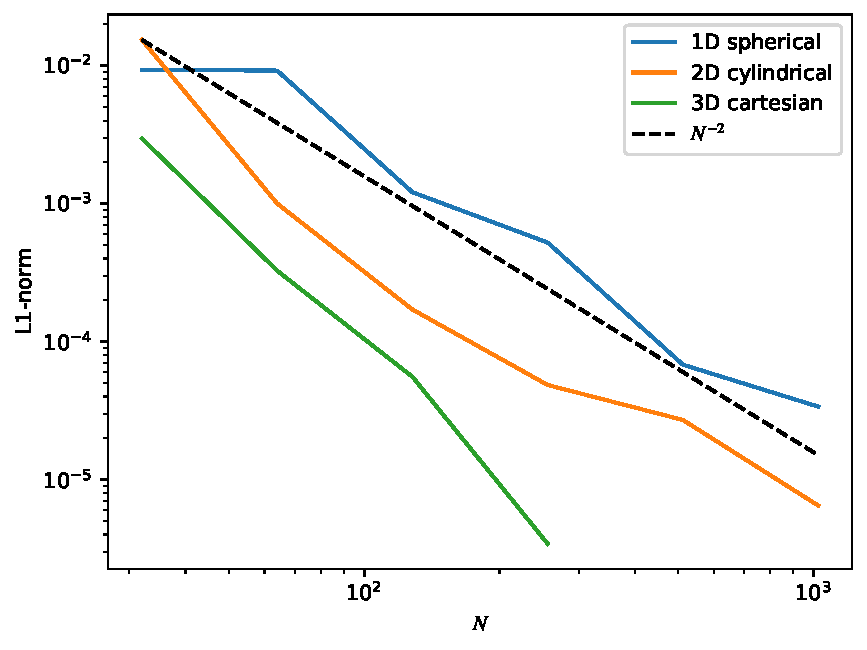
\includegraphics[width=\linewidth]{L1_norm_2.pdf}
  %\caption{A subfigure}
  \label{fig:mg_conv_4}
\end{subfigure}%
\begin{subfigure}{.5\textwidth}
  \centering
  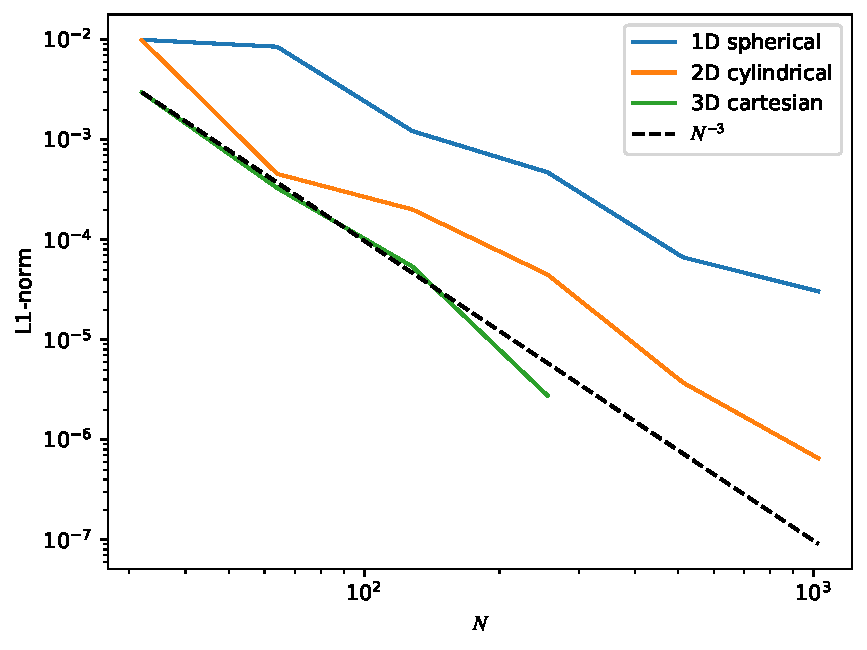
\includegraphics[width=\linewidth]{L1_norm_4.pdf}
  %\caption{A subfigure}
  \label{fig:mg_conv_4}
\end{subfigure}
\caption{L1-norm of $\Phi$ using 2nd order (left) and 4th order central finite difference scheme (right).}
\label{fig:mg_conv}
\end{figure}
Figure \ref{fig:mg_conv} shows the convergent rate of the L1-norm of $\Phi$
\begin{align}
    \left{||} \Phi \right{||}_1 &= \frac{1}{N}\sum^{N}_{i=1} \left| \Phi_i - \Phi^{exact}_i \right|,
\end{align}
where around second-order accuracy and third-order convergence is achieved for 2nd order and 4th order central finite difference scheme in general.

%********************************** %Second Section  *************************************
\section{Teukolsky wave test}
\label{section4.2}
We consider the quadruple $(l,m)=(2,0)$ mode of the vacuum solution.
For even-parity quadruple mode, the metric takes form \cite{teukolsky1982linearized} in spherical coordinate $(r, \theta, \phi)$
\begin{align}
    \begin{split}
    ds^2 =& - dt^2 + \left(1 + A f_{rr}\right) dr^2 + \left(2 B f_{r\theta}\right) r dr d\theta
    + \left(2 B f_{r\phi} \right) r \sin\theta dr d\phi \\
    & \left(1 + C f^{(1)}_{\theta\theta} + A f^{(2)}_{\theta\theta} \right) r^2 d\theta^2
    + \left[2 \left(A-2C\right) f_{\theta\phi} \right] r^2 \sin\theta d\theta d\phi \\
    & + \left(1 + C f^{(1)}_{\phi\phi} + A f^{(2)}_{\phi\phi} \right) r^2 \sin^2\theta d\phi^2,
    \end{split}
\end{align}
where the coefficient $A,B,C$ are constructed from $F(x)$ for $x=t-r$ outgoing wave and $x=t+r$ ingoing wave
\begin{align}
    F(x) = F_1 (t-r) + F_2 (t+r),
\end{align}
and we define
\begin{align}
    F^{(n)} \coloneqq \left. \frac{d^n F_1(x)}{dx^n} \right|_{x=t-r} + (-1)^n \left. \frac{d^n F_2(x)}{dx^n} \right|_{x=t+r}.
\end{align}
Thus, the coefficient are given by
\begin{align}
    A &= 3 \left( \frac{F^{(2)}}{r^3} + \frac{3 F^{(1)}}{r^4} + \frac{3 F}{r^5} \right), \\
    B &= - \left( \frac{F^{(3)}}{r^2} + \frac{3F^{(2)}}{r^3} + \frac{3F^{(1)}}{r^4} + \frac{6F}{r^5} \right), \\
    C &= \frac{1}{4} \left( \frac{F^{(4)}}{r} + \frac{2F^{(3)}}{r^2} + \frac{9F^{(2)}}{r^3} + \frac{21F^{(1)}}{r^4} + \frac{21F}{r^5} \right).
\end{align}
For $m=0$ mode, the angular function $f_{ij}$ are given by
\begin{align}
    f_{rr} &= 2 - 3 \sin^2 \theta, & f_{r\theta} &= - 3 \sin\theta \cos\theta, & f_{r\phi} &= 0, \\
    f_{\theta\theta}^{(1)} &= 3 \sin^2\theta, & f_{\theta\theta}^{(2)} &= -1, & f_{\theta\phi} &= 0, \\
    f_{\phi\phi}^{(1)} &= - f_{\theta\theta}^{(1)}, & f_{\phi\phi}^{(2)} &= 3 \sin^2 \theta - 1.
\end{align}
In our test, we consider 
\begin{align}
    F_1 (x) = - F_2 (x) = \frac{\mathcal{A}}{2} x e^{-\frac{x^2}{\lambda^2}},
\end{align}
and perform the simulation in 2D axisymmetric cylindrical coordinate $(r,z,\phi)$ with $z$ reflection symmetry.
The computational domain covers the region $0\leq \rho \leq 5$, $0\leq z \leq 5$
and the discretization of the domain is set to be $[256,256]$.
The initial profile is given by
\begin{align}\label{eq:Teukolsky_wave_IC}
    \psi &= \alpha = 1, \\
    \beta^i &= 0, \\
    h^{rr} &= \mathcal{A}' \frac{\lambda^4 - \rho^2 z^2}{\lambda^8} e^{-\frac{x^2}{\lambda^2}}, \\
    h^{r z} &= \mathcal{A}' \frac{\rho z \left(\rho^2 - 2 \lambda^2 \right)}{\lambda^8} e^{-\frac{x^2}{\lambda^2}}, \\
    h^{r \phi} &= 0, \\
    h^{zz} &= - \mathcal{A}' \frac{\left(2 \lambda^4 - 4 \lambda^2 \rho^2 + \rho^4 \right)}{\lambda^8} e^{-\frac{x^2}{\lambda^2}}, \\
    h^{z\phi} &= 0, \\
    h^{\phi\phi} &= \mathcal{A}' \frac{\left(\lambda^4 - 4 \lambda^2 \rho^2 +\rho^2 z^2 + \rho^4 \right)}{\lambda^8} e^{-\frac{x^2}{\lambda^2}}, \\
    \hat{A}^{ij} &= 0,
\end{align}
where $\mathcal{A}' = \frac{\mathcal{A}}{12}$.
The analytic solution is written in the Appendix \ref{A3}.
The simulation will be performed under two configurations:
\begin{enumerate}
    %\item Solve the linearized hyperbolic equations only
    %\begin{align}
    %    \partial_t h^{ij} &= 2 \hat{A}^{ij}, \\
    %    \partial_t \hat{A}^{ij} &= \frac{1}{2} f^{kl} \mathcal{D}_k \mathcal{D}_l h^{ij}.
    %\end{align}
    \item Solve the hyperbolic equations only (without elliptic divergence cleaning).
    \label{TW_config_1}
    \item Solve the hyperbolic equations together with the elliptic sector in FCF except $\psi$, $\alpha$ and $\beta$ (with elliptic divergence cleaning).
    \label{TW_config_2}
\end{enumerate}
In the tests, we choose $\mathcal{A}'=10^{-4}$ and $\lambda=1$.
\begin{figure}[h!]
\centering
  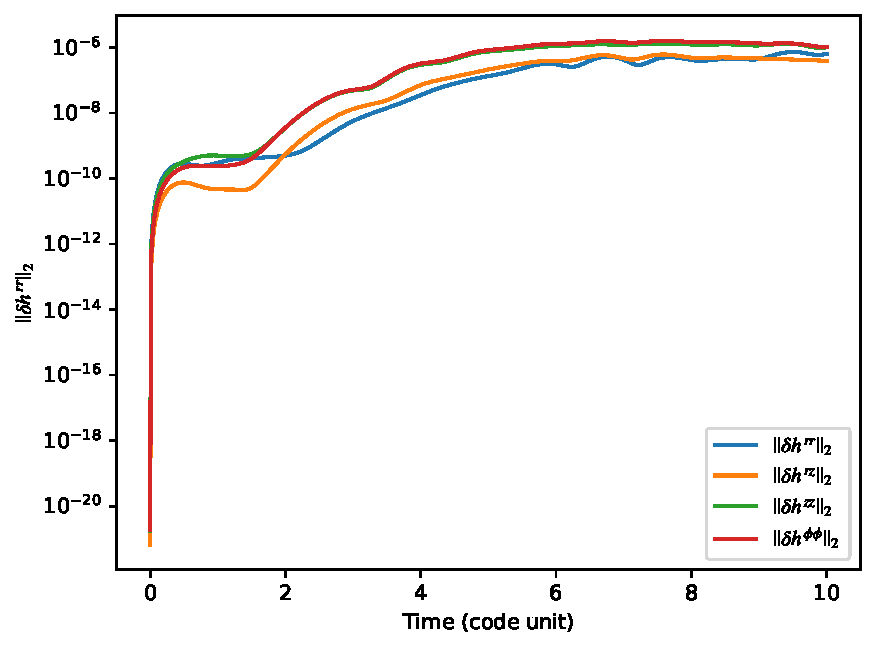
\includegraphics[width=\linewidth]{herr.pdf}
\caption{L2-norm of $h^{ij}$ of the Teukolsky wave test by solving hyperbolic equations without elliptic sector (configuration \ref{TW_config_1}).}
\label{fig:TW_h_err}
\end{figure}
In figure \ref{fig:TW_h_err},
it shows the L2-norm of $h^{ij}$ which is given by
\begin{align}
    \delta h^{ij} &= \sqrt{\frac{1}{V}\sum \left| h^{ij} - h^{ij}_{exact} \right|^2}.
\end{align}
The simulation result agrees with the analytical solution very well.
\begin{figure}[h!]
\centering
\begin{subfigure}{.5\textwidth}
  \centering
  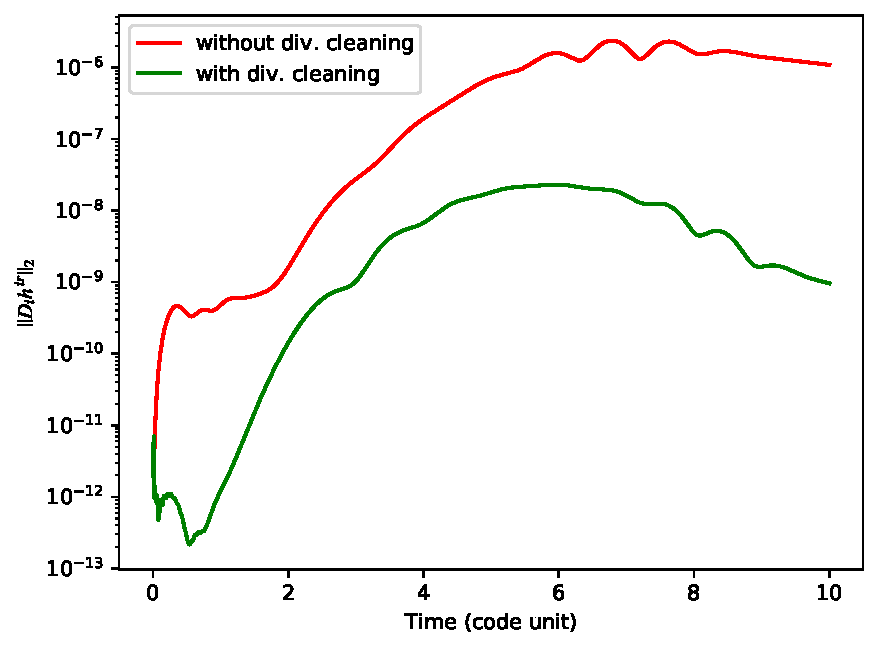
\includegraphics[width=\linewidth]{Dh1.pdf}
  \caption{L2-norm of $\mathcal{D}_i h^{ir}$}
  \label{fig:Dh1}
\end{subfigure}%
\begin{subfigure}{.5\textwidth}
  \centering
  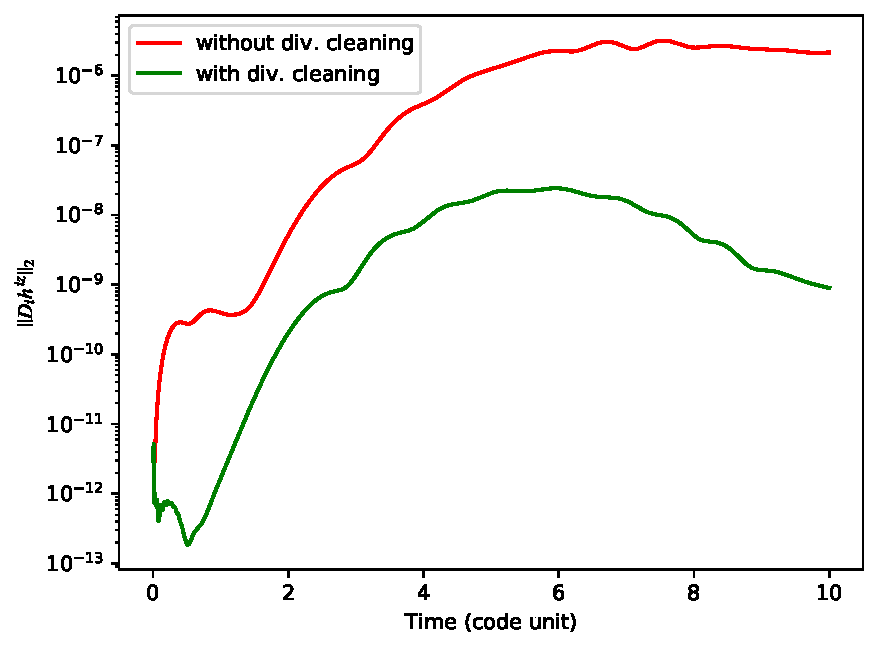
\includegraphics[width=\linewidth]{Dh2.pdf}
  \caption{L2-norm of $\mathcal{D}_i h^{iz}$}
  \label{fig:Dh2}
\end{subfigure}
\caption{L2-norm of the divergence of $h^{ij}$.
The red line corresponds to the evolution of $h^{ij}$ without divergence cleaning
while the green line corresponds to the evolution of $h^{ij}$ with divergence cleaning.}
\label{fig:Dh}
\end{figure}
In figure \ref{fig:Dh}, it shows that the elliptic divergence cleaning method is effective on
reducing the divergence of $h^{ij}$.
Especially for $t \gtrsim 5$ when the wave is propagated out of the computational domain,
the divergence of $h^{ij}$ keep increasing if no treatment is applied,
while it is suppressed with the elliptic cleaning method.
\begin{figure}[h!]
\centering
\begin{subfigure}{.5\textwidth}
  \centering
  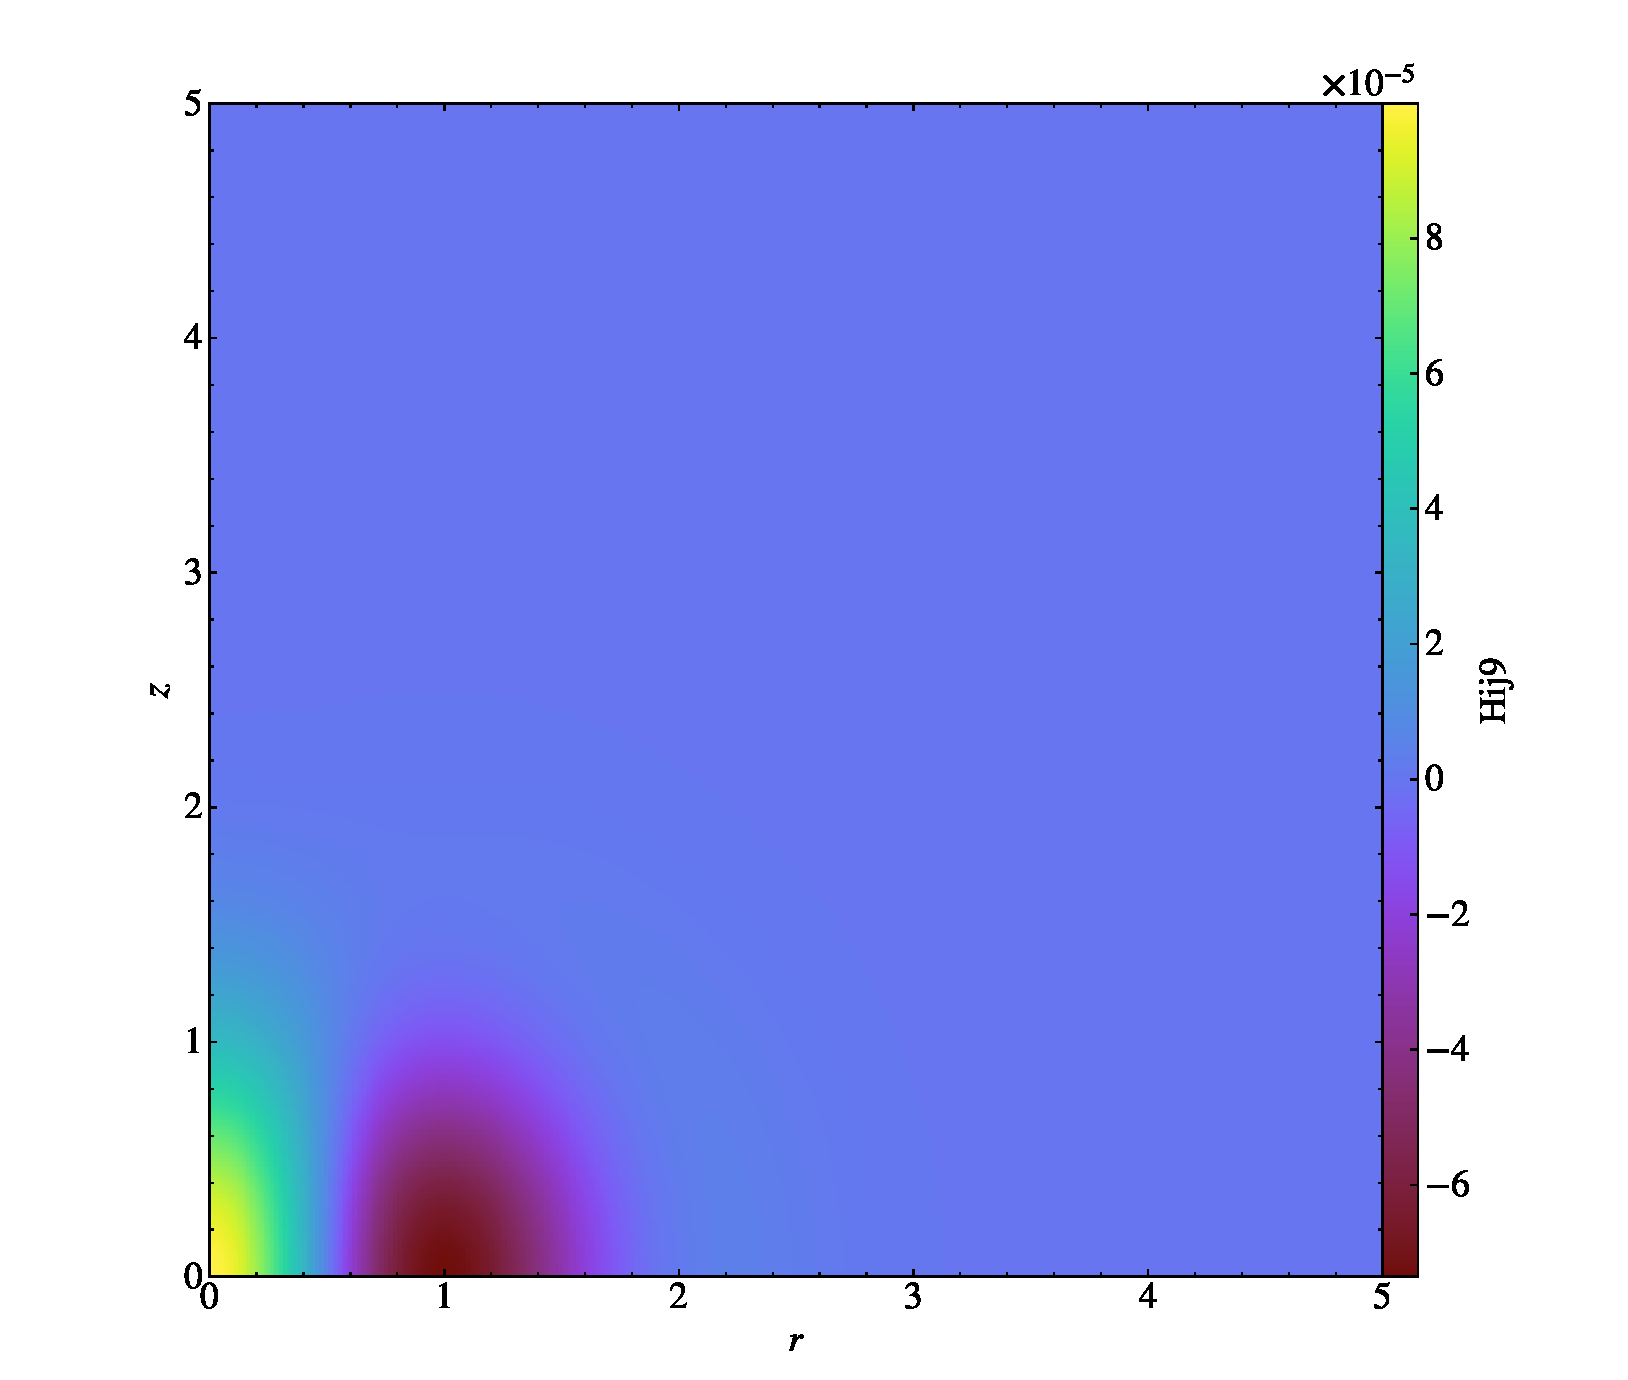
\includegraphics[width=\linewidth]{result_hij_0000.pdf}
  %\caption{L2-norm of $\mathcal{D}_i h^{ir}$}
  \label{fig:hij9_0}
\end{subfigure}%
\begin{subfigure}{.5\textwidth}
  \centering
  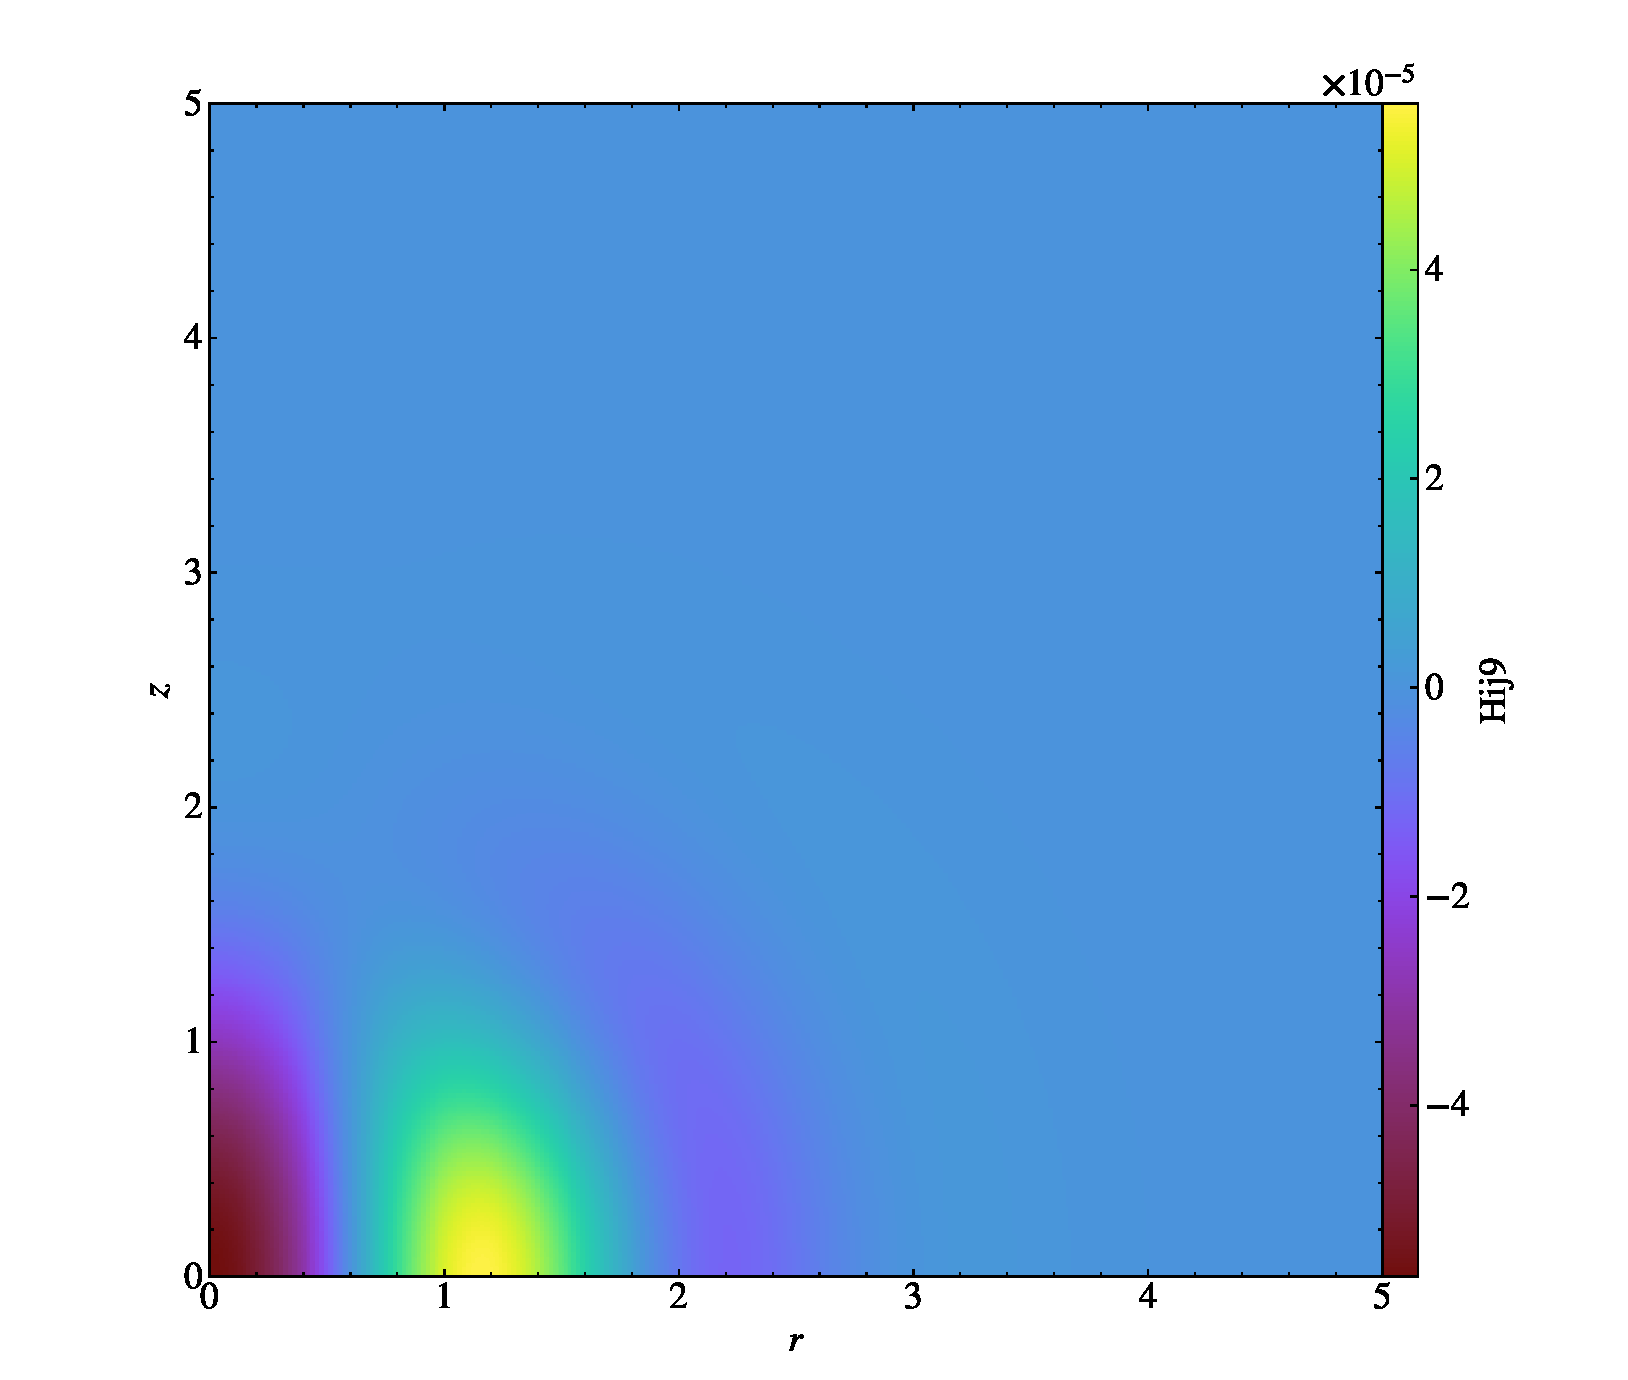
\includegraphics[width=\linewidth]{result_hij_0010.pdf}
  %\caption{L2-norm of $\mathcal{D}_i h^{ir}$}
  \label{fig:hij9_1}
\end{subfigure}%

\begin{subfigure}{.5\textwidth}
  \centering
  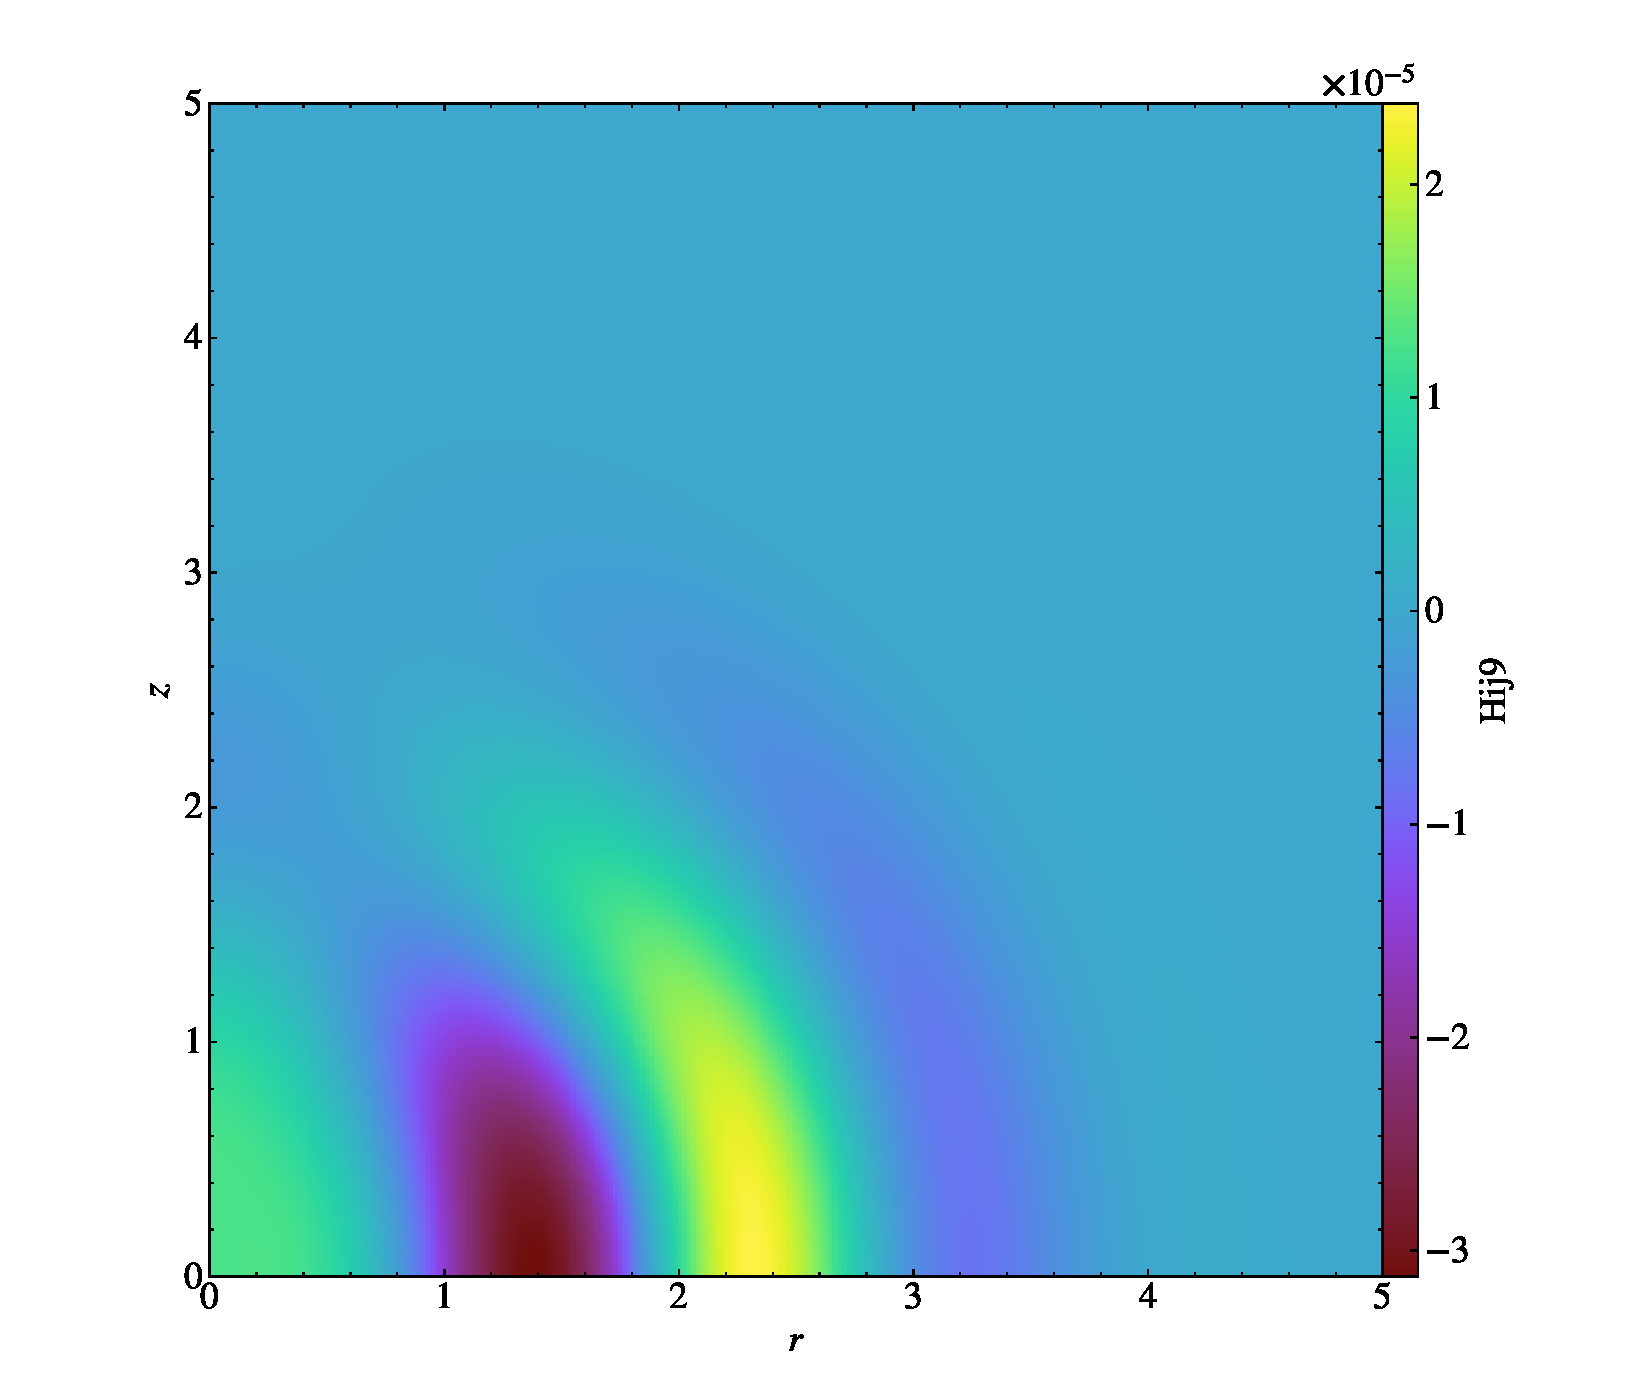
\includegraphics[width=\linewidth]{result_hij_0020.pdf}
  %\caption{L2-norm of $\mathcal{D}_i h^{ir}$}
  \label{fig:hij9_2}
\end{subfigure}%
\begin{subfigure}{.5\textwidth}
  \centering
  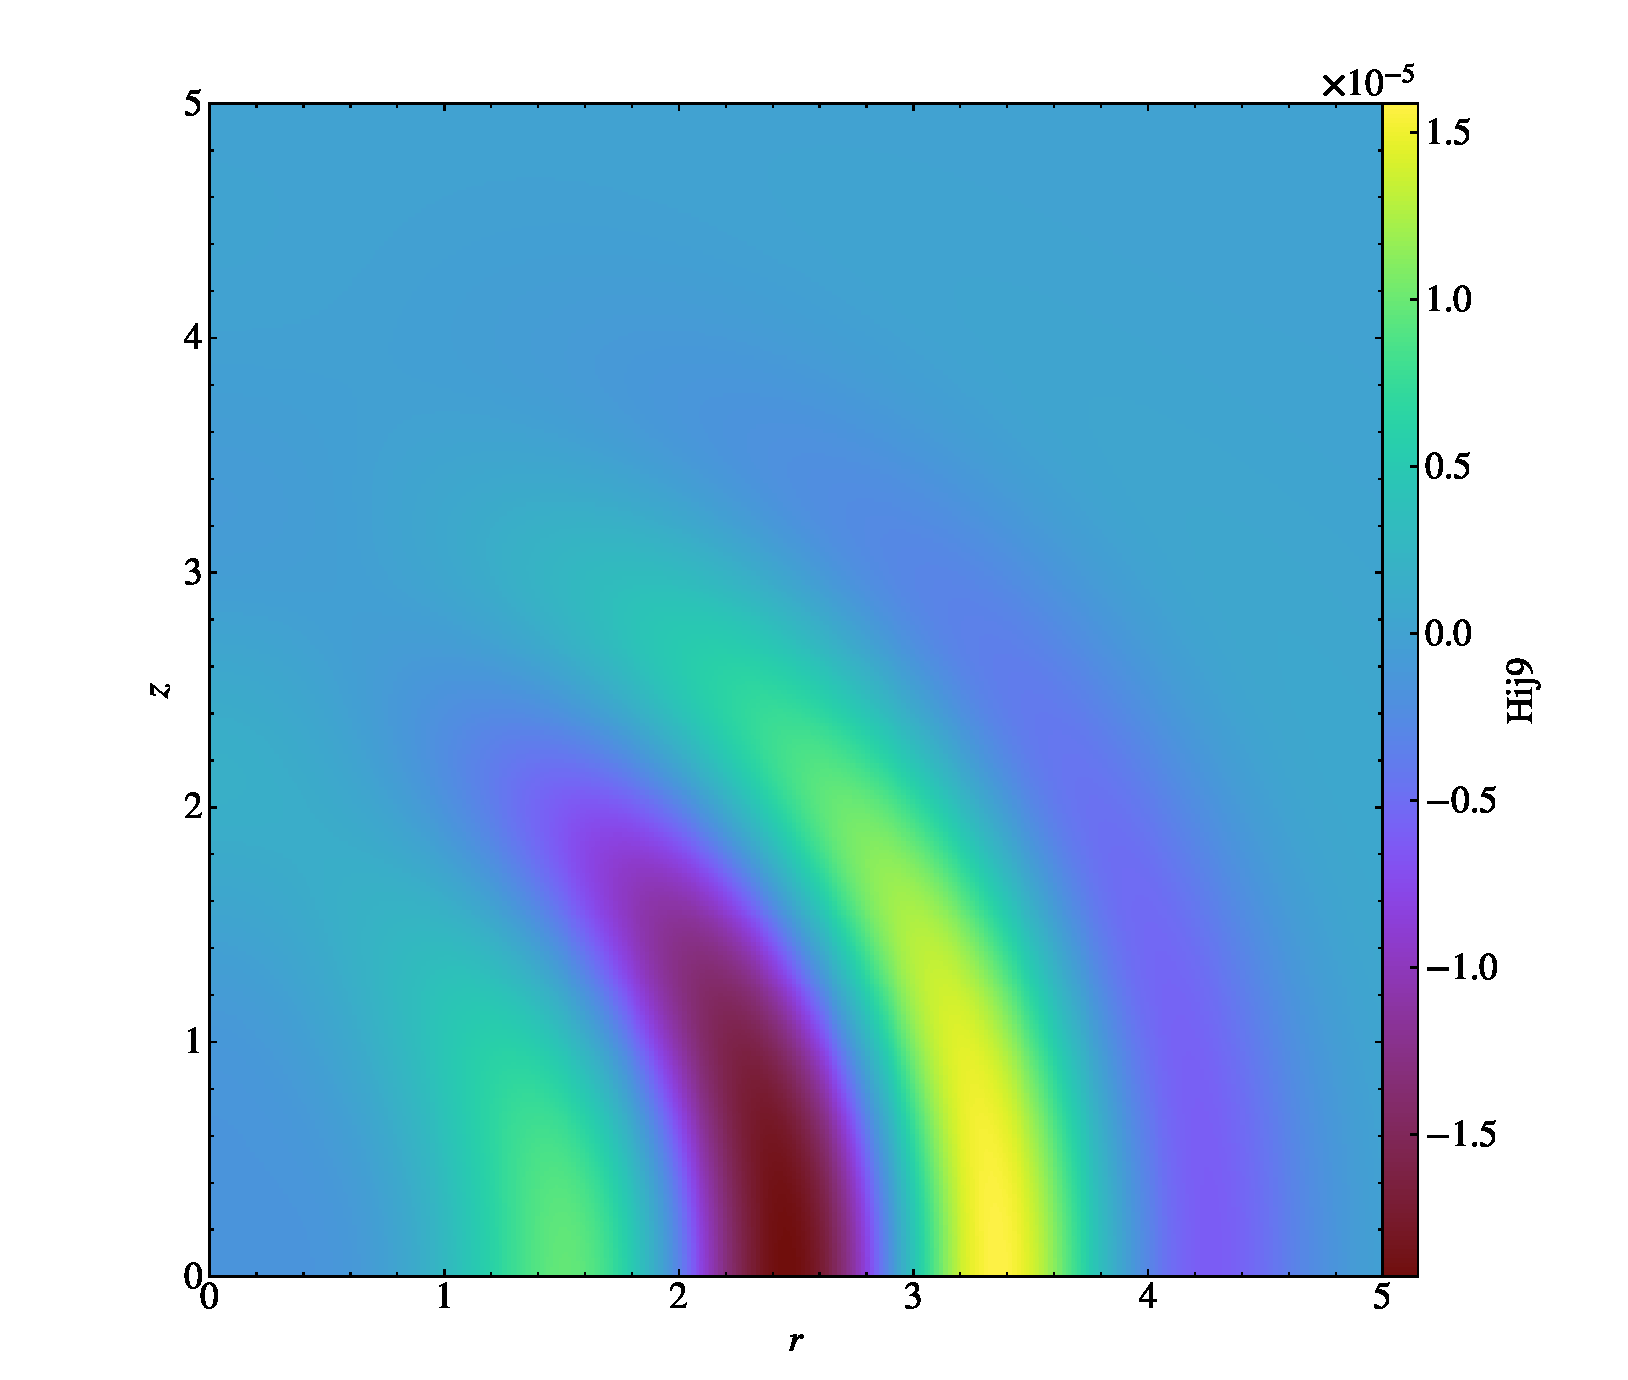
\includegraphics[width=\linewidth]{result_hij_0030.pdf}
  %\caption{L2-norm of $\mathcal{D}_i h^{ir}$}
  \label{fig:hij9_3}
\end{subfigure}%

\begin{subfigure}{.5\textwidth}
  \centering
  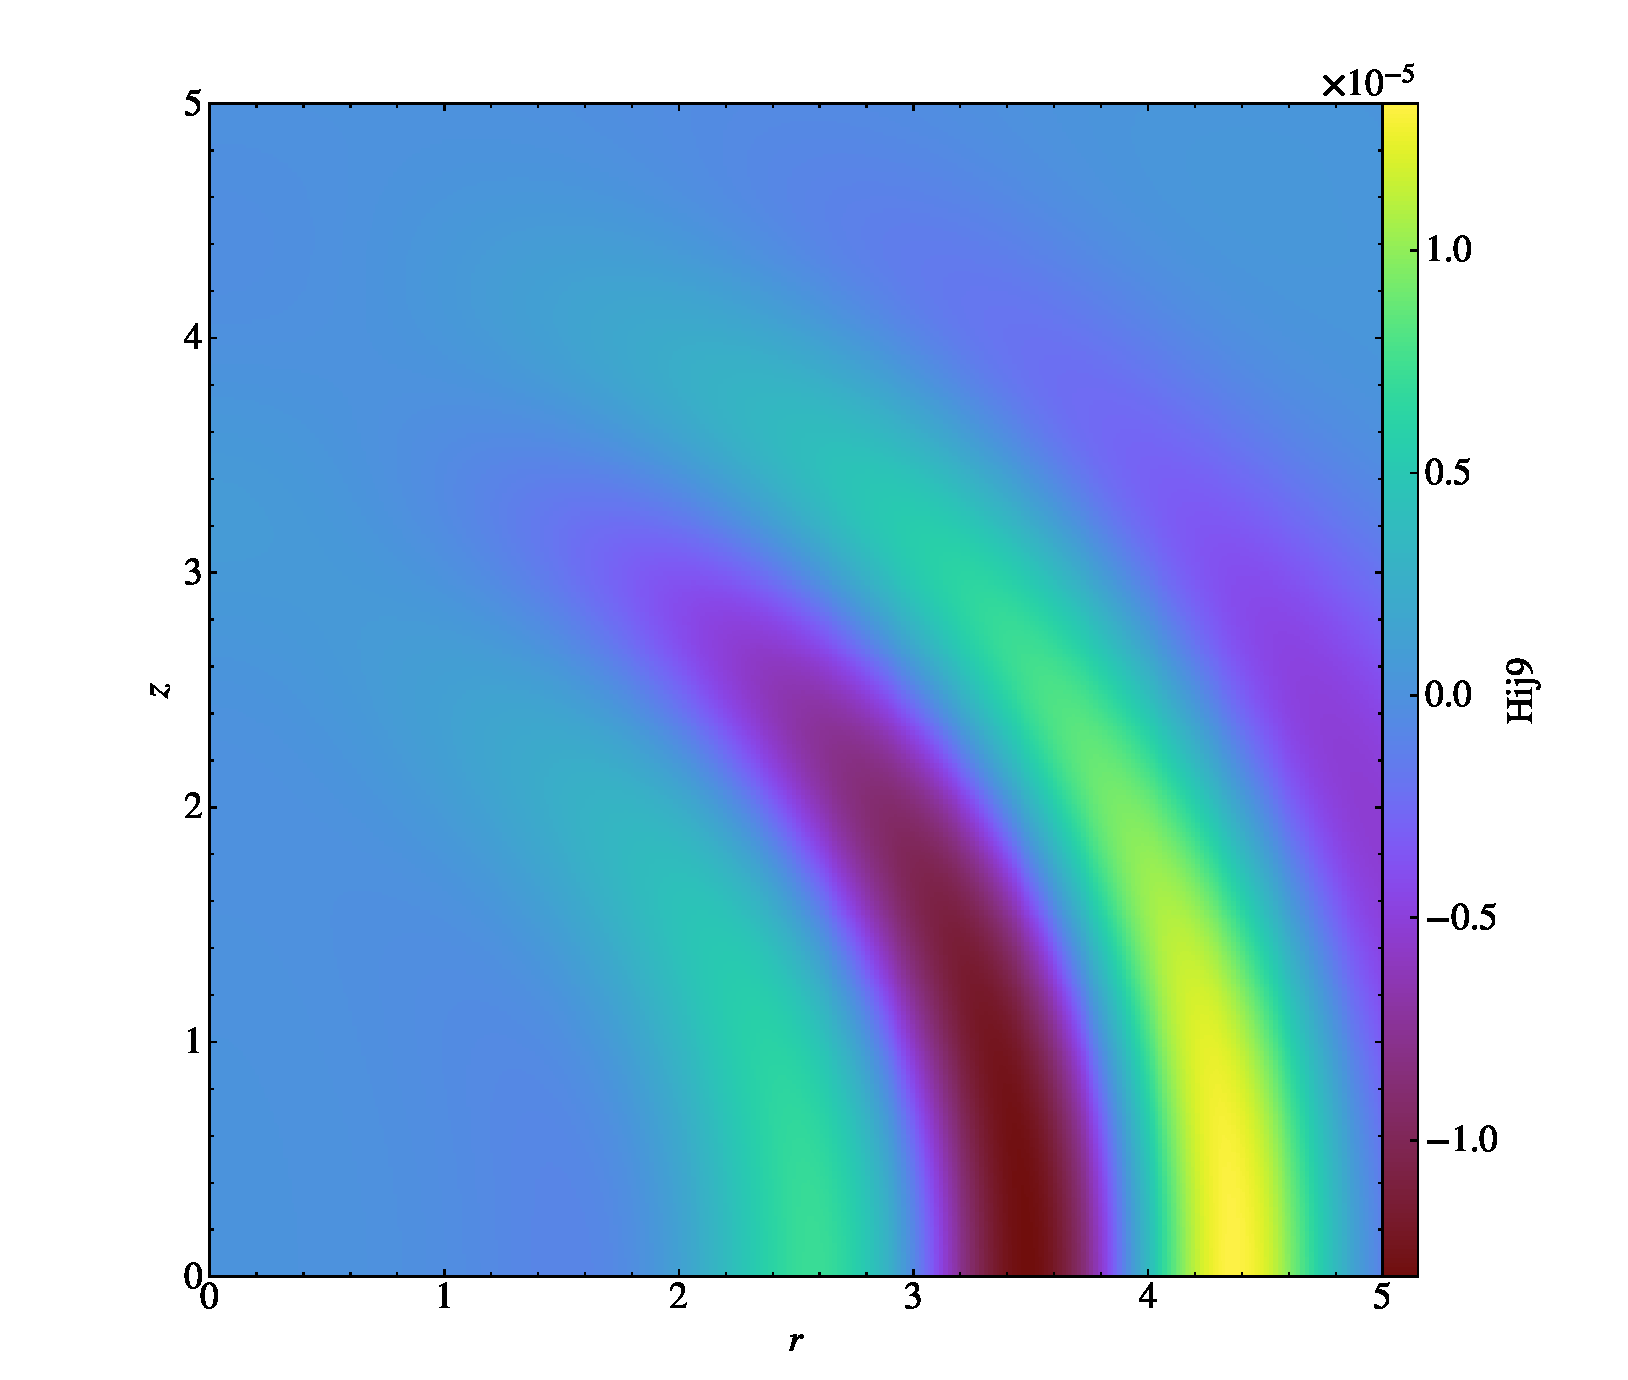
\includegraphics[width=\linewidth]{result_hij_0040.pdf}
  %\caption{L2-norm of $\mathcal{D}_i h^{ir}$}
  \label{fig:hij9_4}
\end{subfigure}%
\begin{subfigure}{.5\textwidth}
  \centering
  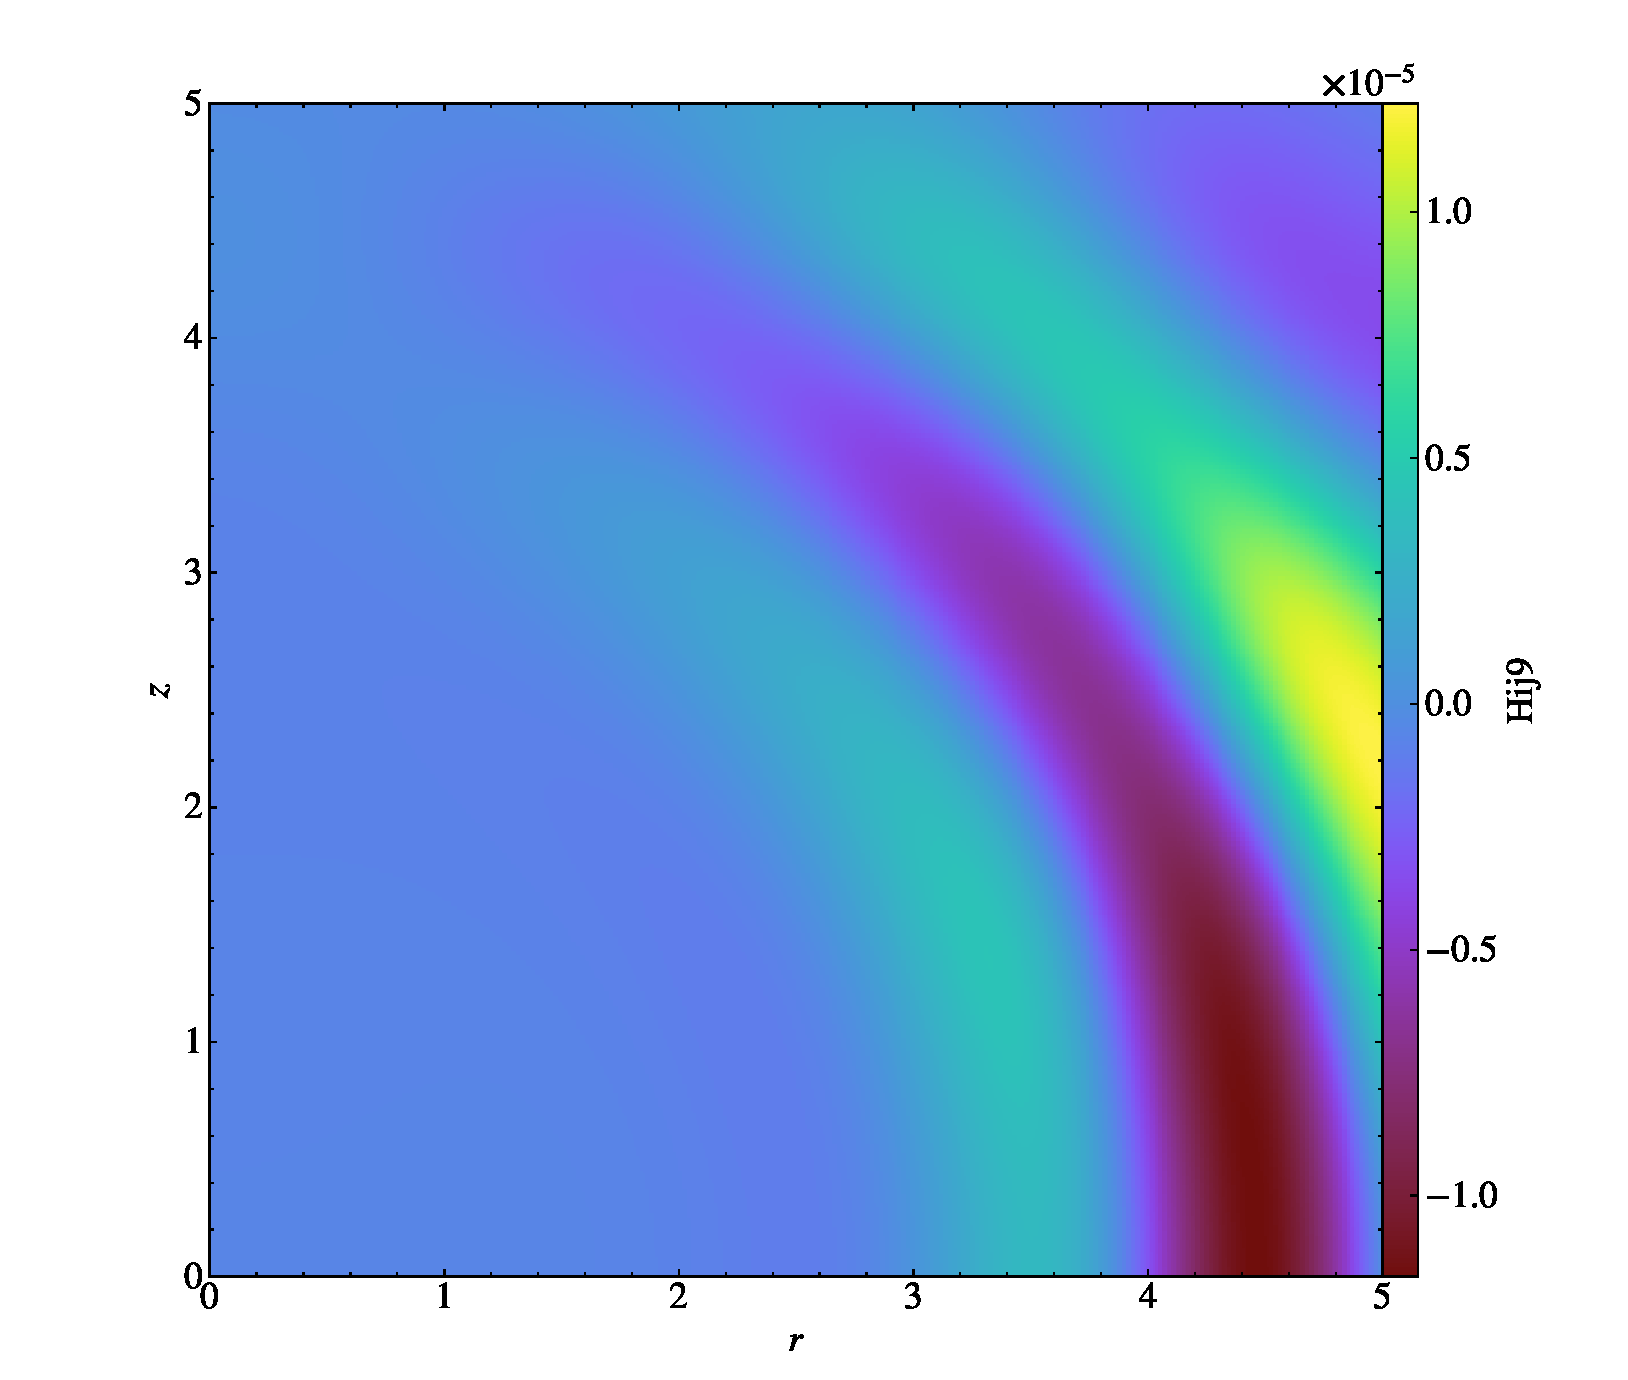
\includegraphics[width=\linewidth]{result_hij_0050.pdf}
  %\caption{L2-norm of $\mathcal{D}_i h^{ir}$}
  \label{fig:hij9_5}
\end{subfigure}%

\caption{Evolution of $h^{\phi\phi}$ component between $t=0$ (upper left) and $t=5$ (lower right) with elliptic divergence cleaning.}
\label{fig:hij9}
\end{figure}
In figure \ref{fig:hij9}, we show the evolution of the $h^{\phi\phi}$ component with elliptic divergence cleaning.

%********************************** %Third Section  *************************************
\section{General relativistic hydrodynamics in dynamic spacetime} %Section - 4.3
\label{section4.3}
Here we study the evolution of a neutron star with dynamical background under FCF scheme and passive FCF scheme.
\subsection{Non-rotating neutron star}
\label{section4.3.1}
In this test, we consider a non-rotating neutron star known as "BU0" \cite{dimmelmeier2006non}
which is constructed with the polytropic index $\Gamma = 2$ and $K = 100$,
and central rest-mass density $\rho_c = 1.28 \times 10^{-3}$ (in $c=G=M_\odot=1$ unit).
This star model is generated by the open-source code \texttt{XNS} 
\cite{bucciantini2011general,pili2014axisymmetric,pili2015general,pili2017general}.
We simulate the star in 2D cylindrical coordinate and impose $z$ reflection symmetry.
The computational domain covers $0 \leq r \leq 60$, $0\leq z \leq 60$ in code unit
with resolution $n_r \times n_z = 256 \times 256$.
The ideal-gas equation of state with $\Gamma = 2$ is used for the simulation.
We extract the plus polarization of gravitational wave signal $h_{+}$ at $(r_{ext}, z_{ext}) = (40, 0)$ which is given by
\begin{align}
    h_{+} \approx \frac{h^{\phi\phi} - h^{zz}}{2} \frac{R_{ext}}{R},
\end{align}
where $R=\sqrt{r^2+z^2}$ is the extraction radius.\\
\begin{figure}[h!]
\centering
  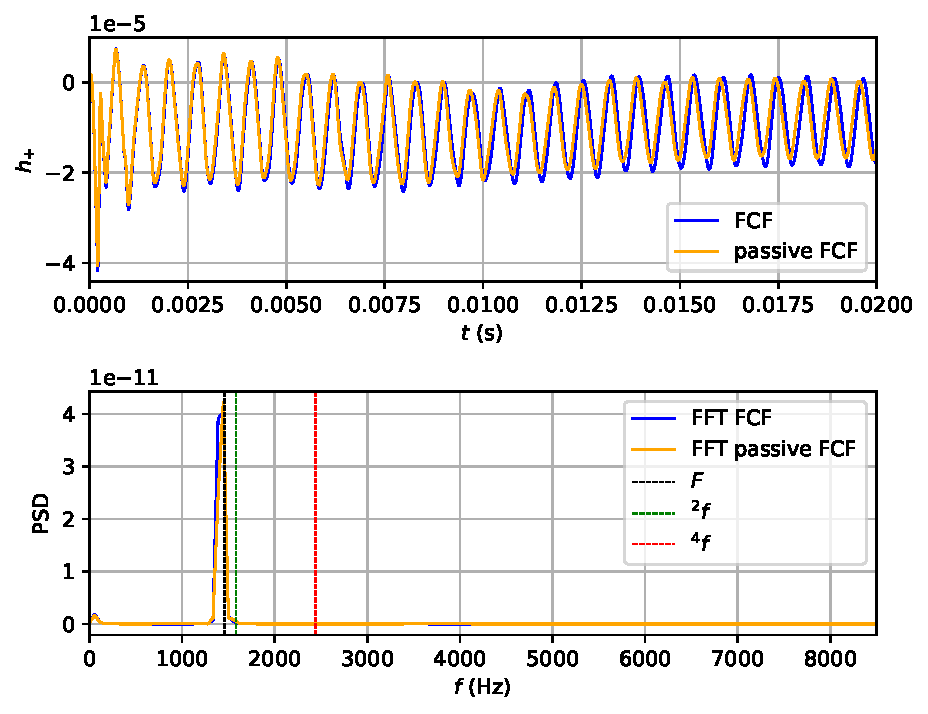
\includegraphics[width=\linewidth]{GW_combine_h_BU0.pdf}
\caption{(upper panel) $h_{+}$ extracted at $(r_{ext}, z_{ext}) = (40, 0)$ from the simulations of oscillating neutron star "BU0".
(lower panel) The power spectral density of $h_{+}$.
The vertical lines represent the known and well-tested eigenmode frequencies \cite{dimmelmeier2006non}}
\label{fig:GW_h_BU0}
\end{figure}
Figure \ref{fig:GW_h_BU0} shows the extracted gravitational wave signal $h_{+}$ from "BU0".
Note that since the BU0 is a spherically symmetric star and it is simulated without any initial perturbation,
only $F$ mode can be extracted which its value agrees with \cite{dimmelmeier2006non}.

\subsection{Rapidly rotating neutron star}
\label{section4.3.2}
In this test, we consider a rapidly-rotating neutron star known as "BU8" \cite{dimmelmeier2006non}.
The polytropic index, $K$ value and central rest-mass density are the same as "BU0",
except that it is uniformly rotating at an angular velocity of $\Omega = 2.633 \times 10^{-2}$.
The simulation setups are same as section \ref{section4.3.1},
and again we extracted $h_{+}$ at $(r_{ext}, z_{ext}) = (40, 0)$.\\
\begin{figure}[h!]
\centering
  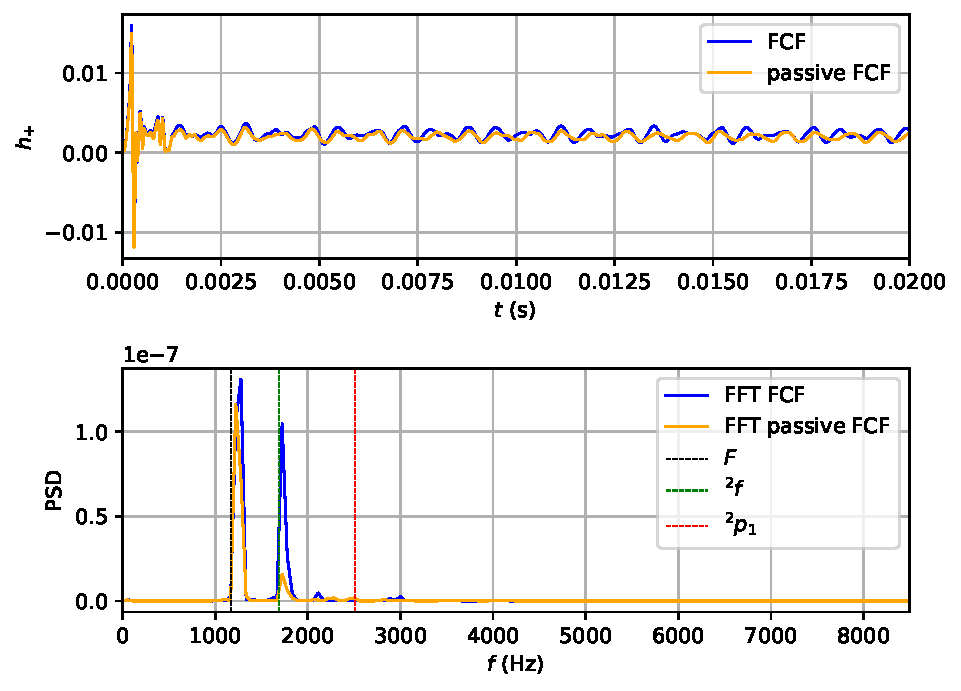
\includegraphics[width=\linewidth]{GW_combine_h_BU8.pdf}
\caption{(upper panel) $h_{+}$ extracted at $(r_{ext}, z_{ext}) = (40, 0)$ from the simulations of oscillating neutron star "BU8".
(lower panel) The power spectral density of $h_{+}$ calculated from $t=2.5ms$ due to the spurious oscillation at the beginning.
The vertical lines represent the known and well-tested eigenmode frequencies \cite{dimmelmeier2006non}}
\label{fig:GW_h_BU8}
\end{figure}
Figure \ref{fig:GW_h_BU8} shows the extracted gravitational wave signal $h_{+}$ from "BU8".
The extracted pulsation mode agrees with \cite{dimmelmeier2006non} for $F$ and ${}^2f$ mode.
Note that the initial profile "BU8" is constructed under CFC approximation with zero $h^{ij}$,
which is not the case when full GR is considered.
This is why a spurious oscillation in $h$ occurs at the beginning of the simulation.
Nonetheless, $h$ quickly settles down and oscillates around the new equilibrium position.
We also observed that the ${}^2f$ mode of $h_+$ in FCF scheme has a higher amplitude compared to passive FCF scheme.

